\documentclass{article}
\usepackage{tikz}
\begin{document}
% 坐标变换. Tikz的图形变化,核心在于坐标的变化,路径的变化也是基于路径上每个点的坐标变化
% 如果需要对tikzpicture环境进行变化,在变化操作后,使用transform shape. 如: \begin{tikzpicture}[scale=0.5,transform shape] ... \end{tikzpicture}
% 路径点无法使用coordinate, transform操作内可以使用coordinate
\begin{tikzpicture}
    % shift - 偏移的位置(x,y). 格式: {<coordinate>}
    % xshift - 在x轴上偏移的位置
    % yshift - 在y轴上偏移的位置
    \draw (0,0) -- (2,0);
    \draw[purple, shift={(-1cm,-1cm)}] (0,0) -- (2,0);
    \draw[red,xshift=1cm] (0,-2) -- (2,-2);
    \draw[green,yshift=-3cm] (0,0) -- (2,0);
\end{tikzpicture}\\\vspace{2cm}

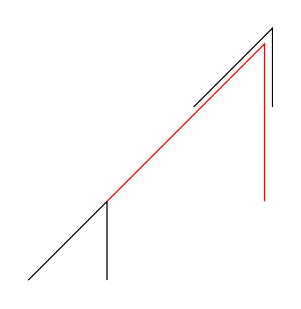
\begin{tikzpicture}
    % scale - 伸缩,所有坐标点乘以伸缩系数
    % scale around - 将指定点视为原点,将其他点坐标与该点的距离进行伸缩. 格式: {<factor>:<coordinate>}
    % xscale - 将坐标的x坐标点进行伸缩
    % yscale - 将坐标的y坐标点进行伸缩
    \draw (1,1) -- (2,2) -- (2,1);
    \draw[shift={(0.1,0.2)}] (3,3) -- (4,4) -- (4,3);
    \draw[red, scale=2] (1,1) -- (2,2) -- (2,1);
\end{tikzpicture}\\\vspace{2cm}

\begin{tikzpicture}
    % rotate - 旋转, 旋转点为(0,0)
    % rotate around - 绕着指定点旋转. 格式: {<degree>:<coordinate>}
    \coordinate (A) at (0,0);
    \coordinate (B) at (4,0);
    \coordinate (C) at (2,0);
    \draw[blue,rotate=60] (0,0) -- (4,0);
    \draw[red,rotate around={90:(C)}] (0,0) -- (4,0);
    \draw (A) -- (B);
\end{tikzpicture}\\\vspace{2cm}

\begin{tikzpicture}
    % xslant - 在x轴方向倾斜factor*y的值
    % yslant - 在y轴方向倾斜factor*x的值
    \draw (0,0) -- (1,1) -- (2,0.75);
    \draw[xslant=2,red] (0,0) -- (1,1) -- (2,0.75);
    \draw[orange] (3,1) circle [radius=2pt];
    \draw[orange] (3.5,0.75) circle [radius=2pt];
    \draw[yslant=2,blue] (0,0) -- (1,1) -- (2,0.75);
    \draw[orange] (1,3) circle [radius=2pt];
    \draw[orange] (2,4.75) circle [radius=2pt];
\end{tikzpicture}\\\vspace{2cm}

\begin{tikzpicture}
    % 变化叠加
    \draw[->] (-3.2,0) -- (3.2,0);
    \draw[->] (0,-3.2) -- (0,3.2);
    \foreach \x in {-3,-2,-1,1,2,3}
      \draw (\x,-1pt) -- (\x,1pt) node[below]{$\x$} (-1pt,\x) -- (1pt,\x) node[left] {$\x$};

    \draw (0,0) -- (1,1) -- (1,0);
    \draw[scale=2,rotate=180,red,thick] (0,0) -- (1,1) -- (1,0);
\end{tikzpicture}
\end{document}
